\documentclass[11pt]{article}
\usepackage[textwidth=18.0cm, textheight=23.0cm, top=2.0cm]{geometry}
\usepackage{pst-all}
\usepackage{amssymb}
\usepackage{tikz}
\usepackage{underscore}\begin{document}
\pagestyle{empty}


ClassName: \underline{\textbf{Class_05.2bp-4}}
\par
BinSize: \underline{\textbf{100 × 100}}
\par
ReduceSize: \underline{\textbf{100 × 100}}
\par
TypeNum: \underline{\textbf{20}}
\par
Num: \underline{\textbf{20}}
\par
OutS: \underline{\textbf{50000}}
\par
InS: \underline{\textbf{43609}}
\par
Rate: \underline{\textbf{0.872}}
\par
UB: \underline{\textbf{5}}
\par
LB0: \underline{\textbf{5}}
\par
LB: \underline{\textbf{5}}
\par
LBWithCut: \underline{\textbf{5}}
\par
NodeCut: \underline{\textbf{0}}
\par
ExtendedNodeCnt: \underline{\textbf{1}}
\par
GenNodeCnt: \underline{\textbf{1}}
\par
PrimalNode: \underline{\textbf{0}}
\par
ColumnCount: \underline{\textbf{5}}
\par
TotalCutCount: \underline{\textbf{0}}
\par
RootCutCount: \underline{\textbf{0}}
\par
LPSolverCnt: \underline{\textbf{1}}
\par
PricingSolverCnt: \underline{\textbf{0}}
\par
BranchAndBoundNum: \underline{\textbf{1}}
\par
isOpt: \underline{\textbf{true}}
\par
TimeOnInitSolution: \underline{\textbf{0.090 s}}
\par
TimeOnPrimal: \underline{\textbf{0.000 s}}
\par
TimeOnPricing: \underline{\textbf{0.000 s}}
\par
TimeOnRmp: \underline{\textbf{0.063 s}}
\par
TotalTime: \underline{\textbf{0.218 s}}
\par
\newpage


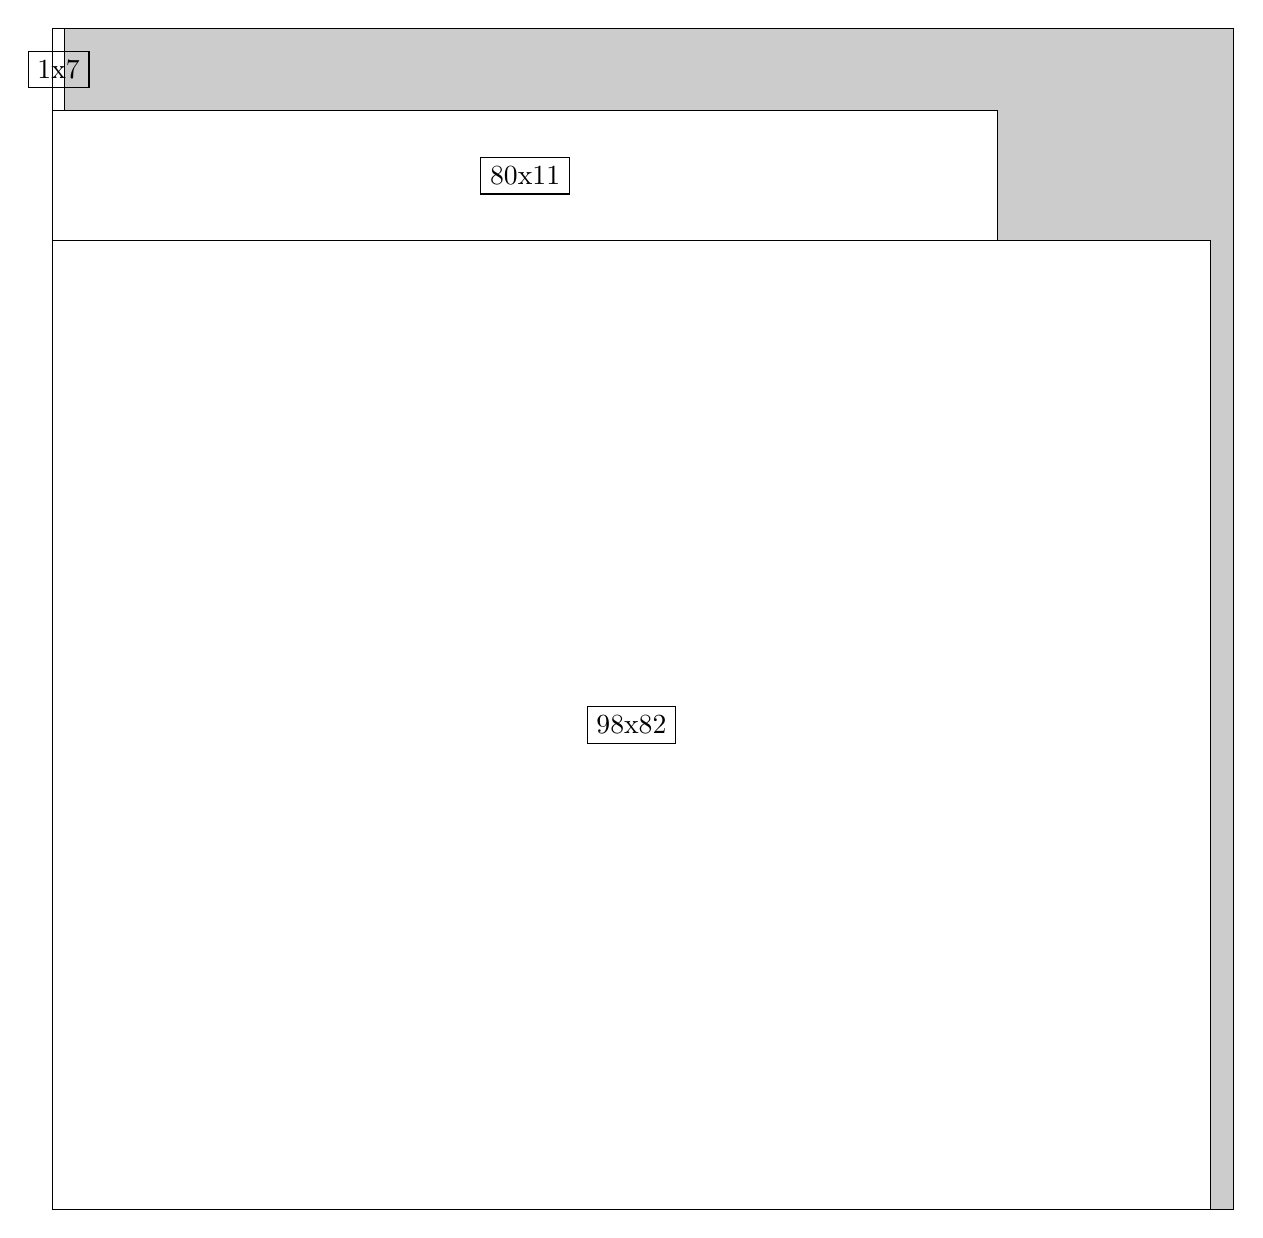
\begin{tikzpicture}[shorten >=1pt,scale=1.0,every node/.style={scale=1.0},->]
\tikzstyle{vertex}=[circle,fill=black!25,minimum size=14pt,inner sep=0pt]
\filldraw[fill=gray!40!white, draw=black] (0,0) rectangle (15.0,15.0);
\foreach \name/\x/\y/\w/\h in {98x82/0.0/0.0/14.7/12.299999999999999,80x11/0.0/12.299999999999999/12.0/1.65,1x7/0.0/13.95/0.15/1.05}
\filldraw[fill=white!40!white, draw=black] (\x,\y) rectangle node[draw] (\name) {\name} ++(\w,\h);
\end{tikzpicture}


w =98 , h =82 , x =0 , y =0 , v =8036
\par
w =80 , h =11 , x =0 , y =82 , v =880
\par
w =1 , h =7 , x =0 , y =93 , v =7
\par
\newpage


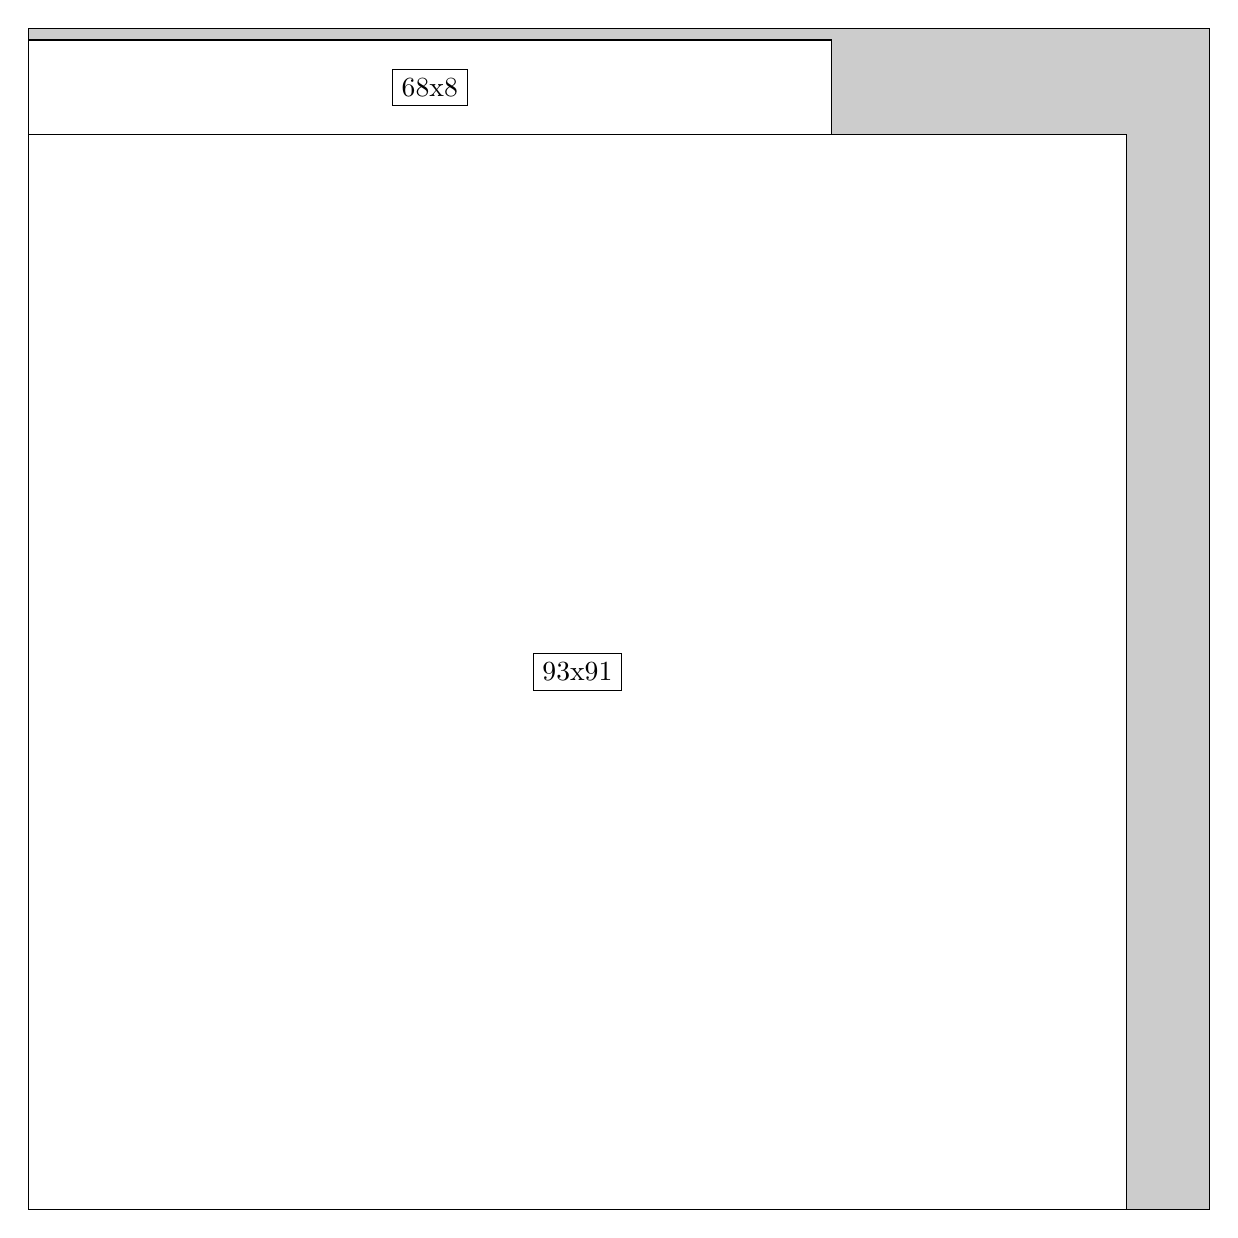
\begin{tikzpicture}[shorten >=1pt,scale=1.0,every node/.style={scale=1.0},->]
\tikzstyle{vertex}=[circle,fill=black!25,minimum size=14pt,inner sep=0pt]
\filldraw[fill=gray!40!white, draw=black] (0,0) rectangle (15.0,15.0);
\foreach \name/\x/\y/\w/\h in {68x8/0.0/13.65/10.2/1.2,93x91/0.0/0.0/13.95/13.65}
\filldraw[fill=white!40!white, draw=black] (\x,\y) rectangle node[draw] (\name) {\name} ++(\w,\h);
\end{tikzpicture}


w =68 , h =8 , x =0 , y =91 , v =544
\par
w =93 , h =91 , x =0 , y =0 , v =8463
\par
\newpage


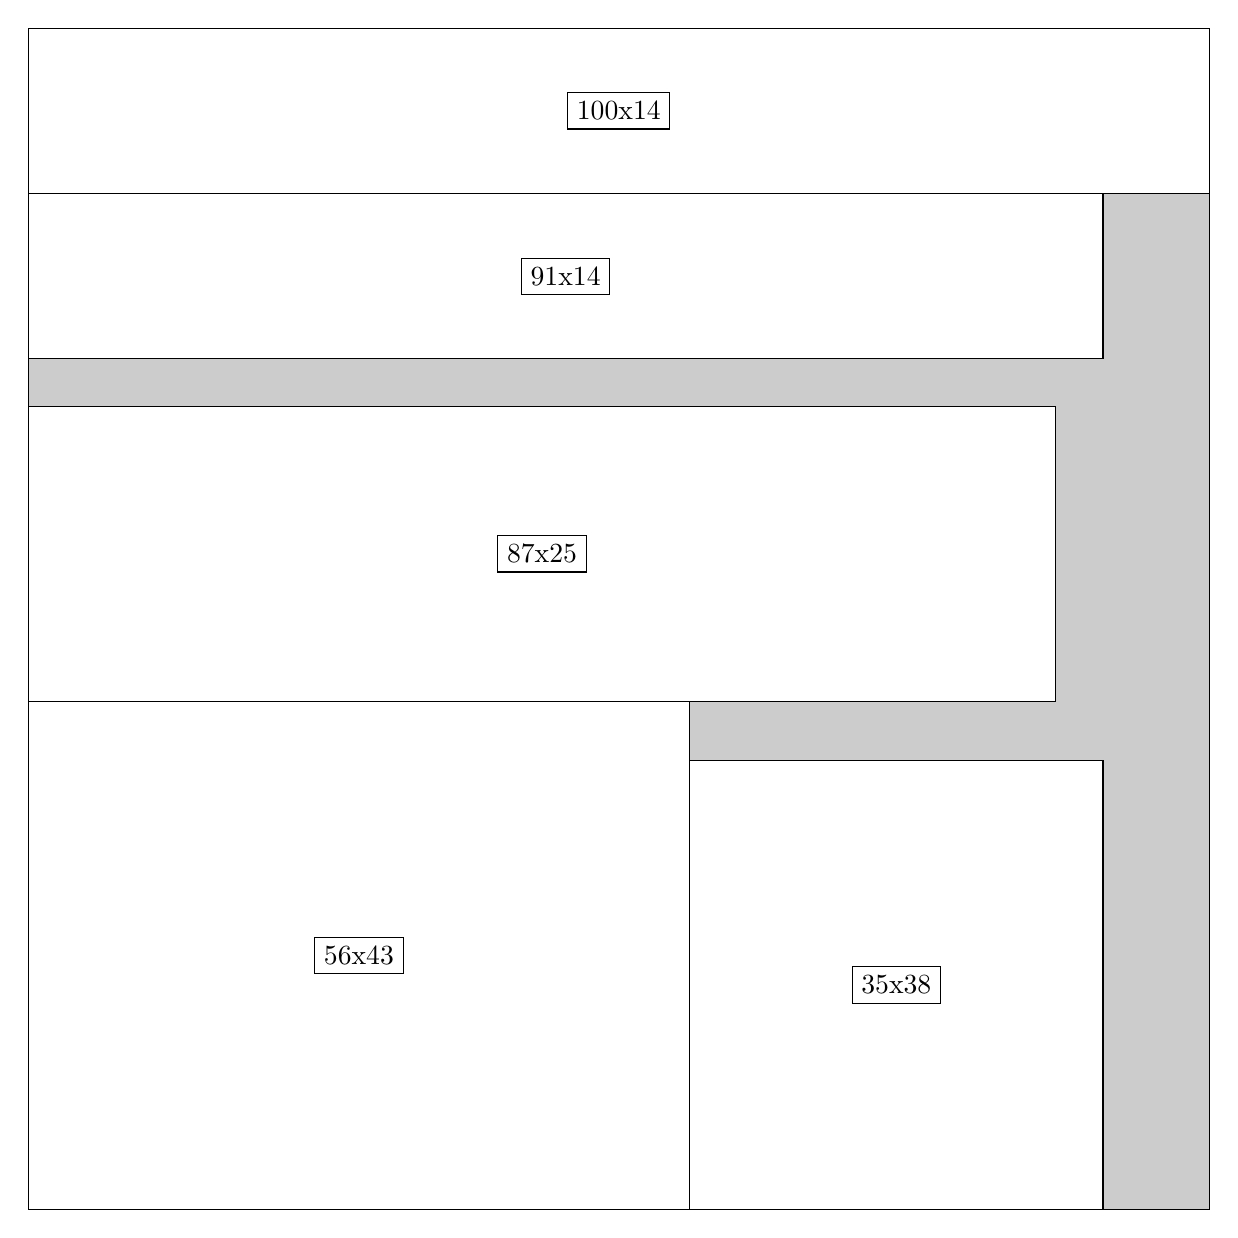
\begin{tikzpicture}[shorten >=1pt,scale=1.0,every node/.style={scale=1.0},->]
\tikzstyle{vertex}=[circle,fill=black!25,minimum size=14pt,inner sep=0pt]
\filldraw[fill=gray!40!white, draw=black] (0,0) rectangle (15.0,15.0);
\foreach \name/\x/\y/\w/\h in {56x43/0.0/0.0/8.4/6.45,87x25/0.0/6.45/13.049999999999999/3.75,100x14/0.0/12.9/15.0/2.1,35x38/8.4/0.0/5.25/5.7,91x14/0.0/10.799999999999999/13.65/2.1}
\filldraw[fill=white!40!white, draw=black] (\x,\y) rectangle node[draw] (\name) {\name} ++(\w,\h);
\end{tikzpicture}


w =56 , h =43 , x =0 , y =0 , v =2408
\par
w =87 , h =25 , x =0 , y =43 , v =2175
\par
w =100 , h =14 , x =0 , y =86 , v =1400
\par
w =35 , h =38 , x =56 , y =0 , v =1330
\par
w =91 , h =14 , x =0 , y =72 , v =1274
\par
\newpage


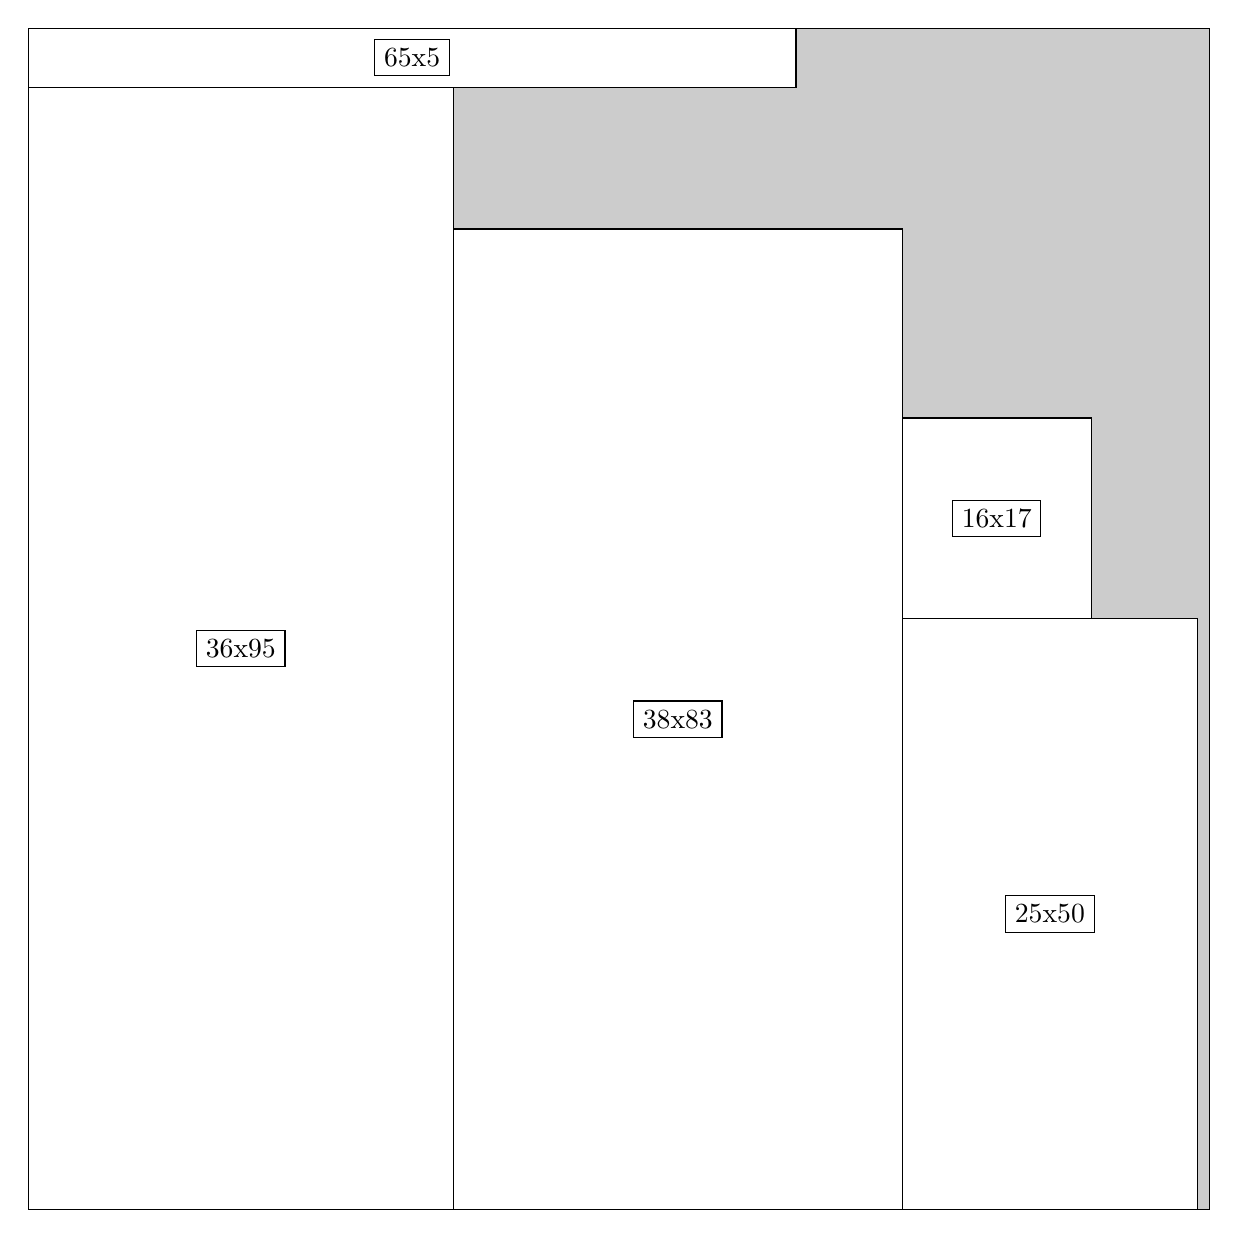
\begin{tikzpicture}[shorten >=1pt,scale=1.0,every node/.style={scale=1.0},->]
\tikzstyle{vertex}=[circle,fill=black!25,minimum size=14pt,inner sep=0pt]
\filldraw[fill=gray!40!white, draw=black] (0,0) rectangle (15.0,15.0);
\foreach \name/\x/\y/\w/\h in {36x95/0.0/0.0/5.3999999999999995/14.25,38x83/5.3999999999999995/0.0/5.7/12.45,25x50/11.1/0.0/3.75/7.5,16x17/11.1/7.5/2.4/2.55,65x5/0.0/14.25/9.75/0.75}
\filldraw[fill=white!40!white, draw=black] (\x,\y) rectangle node[draw] (\name) {\name} ++(\w,\h);
\end{tikzpicture}


w =36 , h =95 , x =0 , y =0 , v =3420
\par
w =38 , h =83 , x =36 , y =0 , v =3154
\par
w =25 , h =50 , x =74 , y =0 , v =1250
\par
w =16 , h =17 , x =74 , y =50 , v =272
\par
w =65 , h =5 , x =0 , y =95 , v =325
\par
\newpage


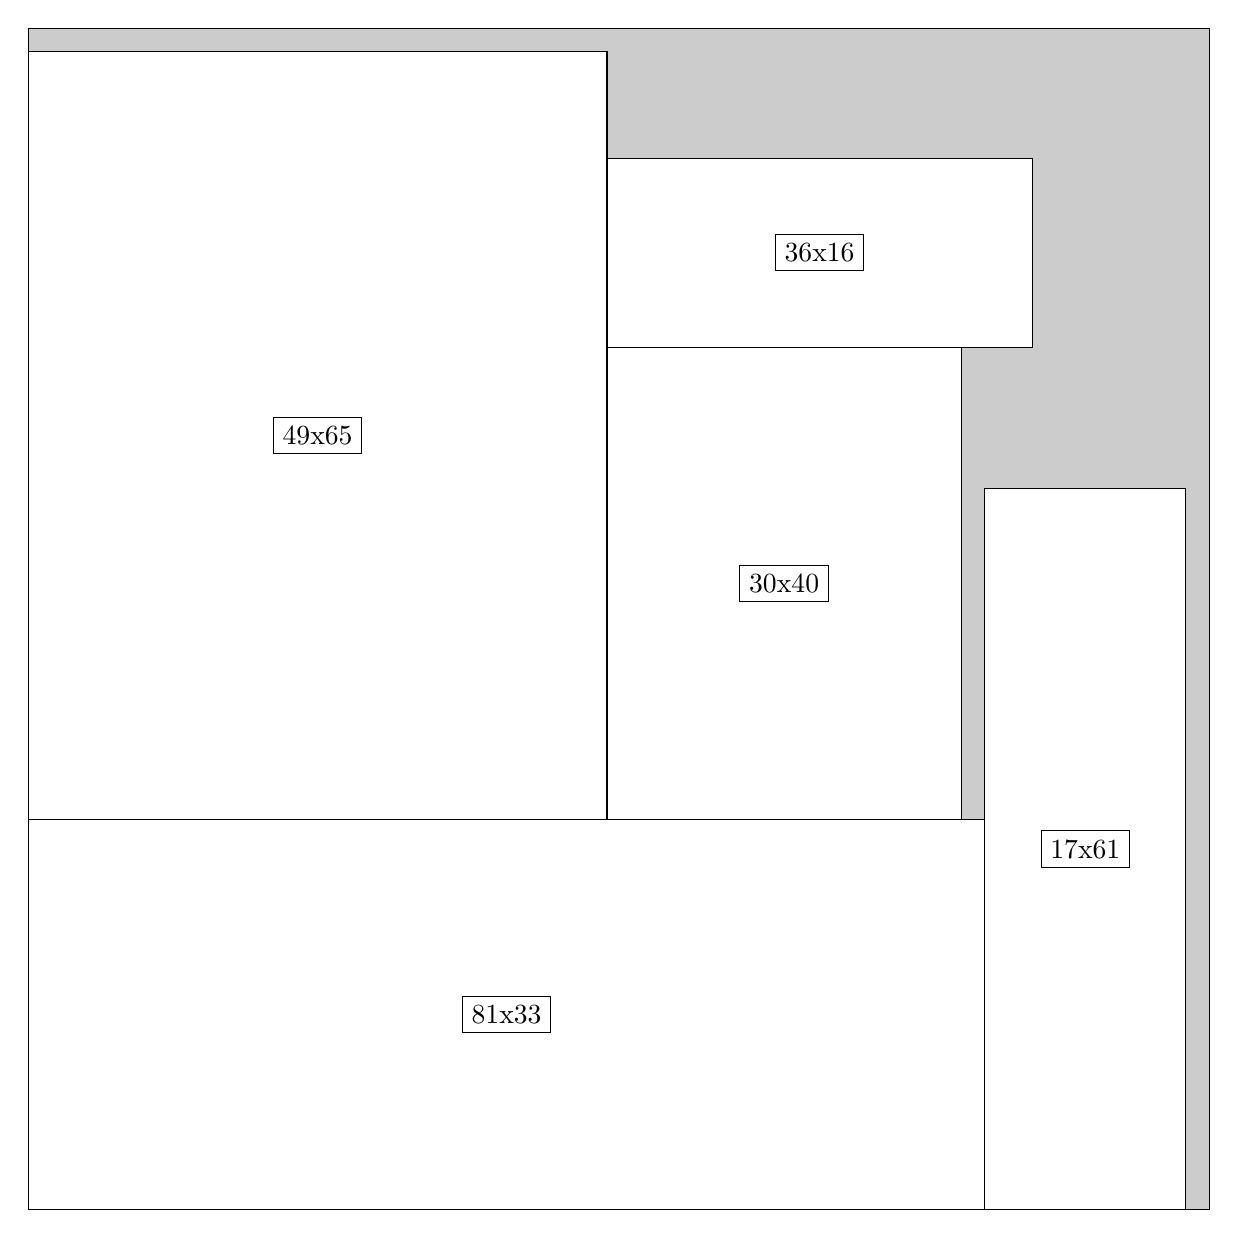
\begin{tikzpicture}[shorten >=1pt,scale=1.0,every node/.style={scale=1.0},->]
\tikzstyle{vertex}=[circle,fill=black!25,minimum size=14pt,inner sep=0pt]
\filldraw[fill=gray!40!white, draw=black] (0,0) rectangle (15.0,15.0);
\foreach \name/\x/\y/\w/\h in {81x33/0.0/0.0/12.15/4.95,49x65/0.0/4.95/7.35/9.75,30x40/7.35/4.95/4.5/6.0,17x61/12.15/0.0/2.55/9.15,36x16/7.35/10.95/5.3999999999999995/2.4}
\filldraw[fill=white!40!white, draw=black] (\x,\y) rectangle node[draw] (\name) {\name} ++(\w,\h);
\end{tikzpicture}


w =81 , h =33 , x =0 , y =0 , v =2673
\par
w =49 , h =65 , x =0 , y =33 , v =3185
\par
w =30 , h =40 , x =49 , y =33 , v =1200
\par
w =17 , h =61 , x =81 , y =0 , v =1037
\par
w =36 , h =16 , x =49 , y =73 , v =576
\par
\newpage


\end{document}